% !TEX root = main.tex

\section{Introduction}
\label{sec:Introduction}

%The weak phase $\gamma$ is the least well known angle of the CKM unitary triangle. 
%A key channel to measure $\gamma$ is the time-dependent analysis of $\Bs\to\Ds\kaon$ decays \cite{Fleischer:2003yb,DeBruyn:2012jp}. 
%The $\Bs\to\Ds\kaon\pion\pion$ proceeds at tree level via the transitions shown in Fig. \ref{fig: BsFeynman} a) and b). 

This note presents the first measurement of the CKM angle $\gamma \equiv \text{arg}[-(V_{ud}V_{ub}^{*})/(V_{cd}V_{cb}^{*})]$ using $\Bs\to\Ds\kaon\pi\pi$ decays, 
where the $\kaon\pion\pion$ subsystem is dominated by excited kaon states such as the $K_{1}(1270)$ and $K_{1}(1400)$ resonances \cite{Blusk:1471393,Blusk:2012it}.
In these decays, sensitivity to the weak phase results from the
interference between $\bquark\to\cquark$ and $\bquark\to\uquark$  transitions achieved through $\Bs-\Bsb$ mixing \cite{Fleischer:2003yb,DeBruyn:2012jp}. 
The amplitudes for both processes are of the same order in the Wolfenstein parameters $\lambda$, $\mathcal O(\lambda^3)$, so that interference
effects are expected to be large. 
The corresponding Feynman diagrams are shown in Fig.~\ref{fig:decay_feynman}.
Due to the interference between mixing and decay amplitudes, the
physical \CP violating observables in these decays are functions of a combination of $\gamma$
and the mixing phase $\beta_s$, namely $\gamma - 2\beta_s$. 
%Again, an amplitude analysis will be crucial in order to determine
%the strong phase difference as function of the phase space, ultimately allowing to separate the weak
%and strong phase contributions.
%To measure the weak CKM phase $\gamma \equiv \text{arg}[-(V_{ud}V_{ub}^{*})/(V_{cd}V_{cb}^{*})]$, a decay with interference between $\bquark\to\cquark$ and $\bquark\to\uquark$ transitions is needed \cite{Fleischer:2003yb,DeBruyn:2012jp}.
%As illustrated in Fig. \ref{fig: BsFeynman}, this is the case for the presented decay mode.  
%It is complementary to the above mentioned analysis of $\Bs\to\Ds\kaon$, making use of a fully charged final state, where every track is detected in the vertex locator. 
To account for the non-constant strong phase across the phase space, 
one can either perform a time-dependent amplitude fit 
%bin the phase space and develop a Dalitz model for each bin, 
or select a suitable phase-space region and introduce a coherence factor as additional hadronic parameter to the decay-time fit.

%This analysis is based on the first observation of the $\Bs\to\Ds\kaon\pion\pion$ decay by LHCb \cite{Blusk:1471393,Blusk:2012it}, where 
%The branching fraction of the $\Bs\to\Ds\kaon\pion\pion$ decay was measured relative to the $\Bs\to\Ds\pion\pion\pion$ decay by LHCb 
%%The result obtained by the previous analysis is 
%$0.052\mbox{ }\pm 0.005\mbox{ } 0.003$, where the uncertainties are statistical and systematical, respectively.  
%The branching ratio measurement is updated, exploiting the full Run 1 data sample, corresponding to 3 $\invfb$ of integrated luminosity.         


\begin{figure}[h]
\centering
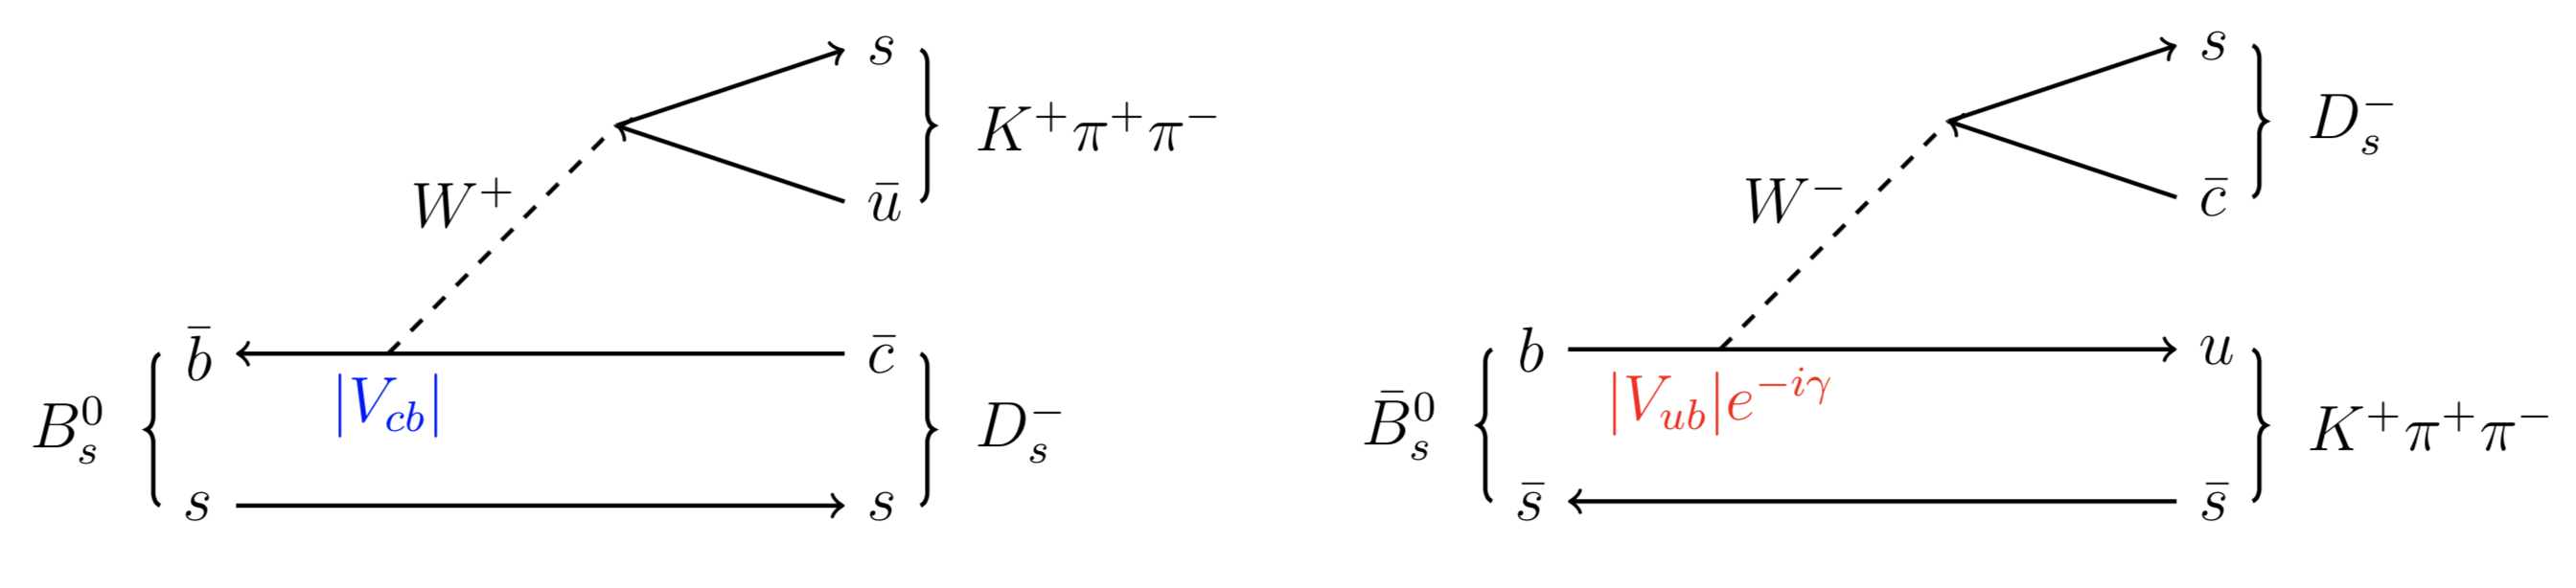
\includegraphics[height=!,width=\textwidth]{figs/feynman.png}
\caption{Feynman diagram for $B_s^0/\bar B_s^0 \to D_s^- K^+ \pip \pim$ decays.}
\label{fig:decay_feynman}
\end{figure}


%\begin{figure}[h]
%\centering
%%\tikzsetnextfilename{feynman_mixing.pdf}
%\begin{tikzpicture}[scale=1.]
%%Strange to beauty quark
%\draw [->,thick] (0,0) node[left]{$s$} -- (4,0) node[right]{$b$};
%%Beauty to strange Anti Quark
%\draw [<-,thick] (0,1) node[left]{$\bar{b}$} -- (4,1) node[right]{$\bar{s}$};
%%W boson
%\draw [dashed,thick] (2.5,0) -- (2.5,1);
%\draw [dashed,thick] (1.5,0) -- (1.5,1);
%
%%Labels
%\draw[decoration={brace},decorate,thick] (-0.5,0) -- node[left=0.2] {$B_s^0$} (-0.5,1);
%\draw[decoration={brace},decorate,thick] (4.5,1) -- node[right=6pt] {$\bar{B}_s^0$} (4.5,0);
%\node at (1.2,0.5) {$W$};
%\node at (2.8,0.5) {$W$};
%\node at (2,-0.3) {$u,c,t$};
%\node at (2,1.3) {$u,c,t$};
%\end{tikzpicture}
%\caption{Feynman diagram of $B_s$ mixing process.}
%\label{fig:mixing_feynman}
%\end{figure}
%
%
%\begin{figure}[h]
%\centering
%   
%\begin{subfigure}[b]{0.45\textwidth}
%
%\begin{tikzpicture}[scale=1]
%%Strange quark
%\draw [->,thick] (0,0) node[left]{$s$} -- (4,0) node[right]{$s$};
%%Beauty to Charm Quark
%\draw [<-,thick] (0,1) node[left]{$\bar{b}$} -- (4,1) node[right]{$\bar{c}$};
%\node at (1.,0.66) {$\textcolor{blue}{\vert V_{cb} \vert}$};
%
%%W+ boson
%\draw [dashed,thick] (1,1) -- (2.5,2.5);
%\node at (1.5,2) {$W^+$};
%%u Quark
%\draw [->,thick] (2.5,2.5) -- (4,3) node[right]{$s$};
%%d Quark
%\draw [<-,thick](2.5,2.5) -- (4,2) node[right]{$\bar{u}$};
%
%%pipipi brace and node
%\draw[decoration={brace},decorate,thick](4.5,3) -- node[right=6pt] {$K^+\pi^+\pi^-$} (4.5,2);
%%Ds brace and node
%\draw[decoration={brace},decorate,thick] (4.5,1) -- node[right=6pt] {$D_s^-$} (4.5,0);
%%Bs brace and node
%\draw[decoration={brace},decorate,thick] (-0.5,0) -- node[left=0.2] {$B_s^0$} (-0.5,1);
%\end{tikzpicture}
%
%\end{subfigure} \hfill
%%
%%
%%
%%
%%
%\begin{subfigure}[b]{0.45\textwidth}
%
%\begin{tikzpicture}[scale=1]
%%Strange quark
%\draw [<-,thick] (0,0) node[left]{$\bar s$} -- (4,0) node[right]{$\bar s$};
%%Beauty to Charm Quark
%\draw [->,thick] (0,1) node[left]{$b$} -- (4,1) node[right]{$u$};
%\node at (1.,0.66) {$\textcolor{red}{\vert V_{ub} \vert e^{-i\gamma}}$};
%%W+ boson
%\draw [dashed,thick] (1,1) -- (2.5,2.5);
%\node at (1.5,2) {$W^-$};
%%u Quark
%\draw [->,thick] (2.5,2.5) -- (4,3) node[right]{$s$};
%%d Quark
%\draw [<-,thick](2.5,2.5) -- (4,2) node[right]{$\bar{c}$};
%
%%pipipi brace and node
%\draw[decoration={brace},decorate,thick](4.5,3) -- node[right=6pt] {$D_s^-$} (4.5,2);
%%Ds brace and node
%\draw[decoration={brace},decorate,thick] (4.5,1) -- node[right=6pt] {$K^+\pi^+\pi^-$} (4.5,0);
%%Bs brace and node
%\draw[decoration={brace},decorate,thick] (-0.5,0) -- node[left=0.2] {$\bar B_s^0$} (-0.5,1);
%\end{tikzpicture}
%
%\end{subfigure}
%\caption{Feynman diagram for $B_s^0/\bar B_s^0 \to D_s^- K^+ \pip \pim$ decays.}
%\label{fig:decay_feynman}
%
%\end{figure}